\chapter{Analytic Evaluation of the Effective Theory} \label{chap5}

In \chapref{chap4} we introduced the dimensionally reduced effective theory for
heavy quarks at strong coupling. We ended the chapter with a section on the
numerical handling of the theory and its advantages over full lattice gauge
theory simulations. Although a lot of progress has been made evaluating the
predictions of the theory \citep{Fromm:2011qi,Fromm:2012eb,Langelage:2014vpa},
we see from the convergence plots in \figref{fig:numerical_convergence} that
convergence is slow and other approaches should be considered.

It was observed in one of the previous studies of the effective theory
\citep{Langelage:2014vpa} that it is possible to treat the effective theory
purely analytical which provides a plethora of useful methods which we will
explore in this chapter. First and foremost it lends insight into the
mathematical and physical structure of the effective theory and serves as a
cross check for the numerical methods. In \secref{sec:cluster_expansion} we will
present the linked cluster expansion which will provide the building blocks for
a systematic study of the analytic evaluation. We will see how one can translate
between the language of spin statistics and nearest neighbour systems and the
strong coupling, heavy quark formalism. In \secref{sec:analytic_resummation} we
will introduce a new resummation scheme to the analytic evaluation which is
inaccessible to numerical methods. To do this we will exploit the care we put
into the section on effective theory combinatorics.

In \secref{sec:evaluation} we will utilise the full power of the analytic
expressions to study the various aspects of the theory at hand, comparing with
numerical results, studying lattice artefacts and more.

Finally in \secrefs{sec:large_nc_study,sec:yang_lee_zeros} we carry out two
exploratory studies in which the analytic evaluation is paramount. Although
these still pose a lot of open questions, we will build foundations on which
future studies can be performed.

\section{Linked cluster expansion} \label{sec:cluster_expansion}

We start once more on a more fundamental level by introducing the linked cluster
formalism for scalar fields with nearest neighbour interactions. Although the
following section to a sense should be complete, we refer to introductory texts
on the subject for more details, e.g. \citep{Wortis:1980zb,Reisz:1995ag}, and
\citep{Domb:1980zb,Martin:1980zb} for a physics focused presentation of simple
graph theoretical practices. After the fundamentals are out of the way we study
how one can expand the formalism to also include $n$-point interactions with
finite spatial extent, a formalism in which the effective theory can then be
expressed.

\subsection{Classical linked cluster expansion for nearest neighbour interactions}

To introduce the framework we consider a scalar field with a $2$-point coupling
%
\begin{equation}
  \mathcal{Z} = \int [\mathrm{d} \phi] e^{-S_0[\phi] + \frac{1}{2} \sum_{x,y}
    \phi(x) v(x,y) \phi(y)},
\end{equation}
%
where function $v(x,y)$ encodes the coupling information.We will assume that the
coupling strength is small enough to justify an expansion around the free
theory. To facilitate the expansion we introduce source fields $J(x)$ and define
the generating functional
%
\begin{equation}
  \mathcal{Z}[J] = \int [\mathrm{d} \phi] e^{-S[\phi] + \sum_x J(x) \phi(x)}.
\end{equation}
%
Since our goal is to study thermodynamic quantities, we shift our attention to
the computation of the free energy $\mathcal{W}$, or the generating functional
of connected correlation functions
%
\begin{equation}
  \mathcal{W}[J,v] = - \log \mathcal{Z}[J,v].
\end{equation}
%
A linked cluster expansion of the free energy is then defined as the Taylor
expansion with respect to the coupling $v(x,y)$ around the free theory
%
\begin{equation} \label{eq:cluster_expansion_def}
  \mathcal{W}[J,v] = \bigg( \exp \bigg(\frac{1}{2} \sum_{x,y} v(x,y)
    \frac{\delta}{\delta \hat{v}(x,y)} \bigg) \bigg) \mathcal{W}[J,\hat{v}]
    \,\Bigg|_{\hat{v}=0}.
\end{equation}
%
One can rewrite the derivative of $\mathcal{W}$ with respect to the couplings in
terms of derivatives with respect to the sources
%
\begin{equation}
  \frac{\delta \mathcal{W}}{\delta v(x,y)} = \frac{\delta^2 \mathcal{W}}{\delta
    J(x) \delta J(y)} + \frac{\delta \mathcal{W}}{\delta J(x)} \frac{\delta \mathcal{W}}{\delta J(y)}.
\end{equation}
%
We also know that $\mathcal{W}[J]$ is the generating functional of the
connected $n$-point functions 
%
\begin{equation}
  \frac{\delta \mathcal{W}}{\delta J(x)} \bigg|_{J=\mathrlap{0}} 
    = \frac{1}{\mathcal{Z}} \int [\mathrm{d} \phi] \, \phi(x) \, e^{-S[\phi]}
    \equiv \langle \phi(x) \rangle,
\end{equation}
%
which for higher order derivatives produces the cumulants
%
\begin{equation}
  \frac{\delta^2 \mathcal{W}}{\delta J(x) \delta J(y)} \bigg|_{J=\mathrlap{0}} 
    = \langle \phi(x) \phi(y) \rangle - \langle \phi(x) \rangle \langle \phi(y) \rangle.
\end{equation}
%
To second order the expansion in \meqref{eq:cluster_expansion_def} is
%
\begin{multline} \label{eq:linked_cluster_2nd_order}
  \mathcal{W}[J, v] = \mathcal{W}[J,0]
    + \frac{1}{2} \sum_{x,y} v(x,y) \frac{\delta \mathcal{W}[J,\hat{v}]}{\delta \hat{v}(x,y)} \bigg|_{\hat{v}=0} \\
    + \frac{1}{8} \sum_{x,y} \sum_{z,w} v(x,y) v(z,w) \frac{\delta^2
      \mathcal{W}[J,\hat{v}]}{\delta \hat{v}(x,y) \delta \hat{v}(z,w)}
    \bigg|_{\hat{v}=0} + \dots
\end{multline}
%
We define the coupled $n$-point functions by
%
\begin{equation}
  \mathcal{M}_n(x_1, x_2, \dots, x_n) = \frac{\delta^n \mathcal{W}[J,v]}{\delta
    J(x_1) \delta J(x_2) \cdots \delta J(x_n)}
\end{equation}
%
which in turn define the free theory $n$-point functions
%
\begin{equation}
   \mathcal{M}_n(x_1, x_2, \dots, x_n) \big|_{v = 0}
   = M_n(x_1) \delta(x_1, x_2, \dots, x_n)
\end{equation}
%
where the Kronecker deltas naturally arise in the free theory
%
\begin{equation}
  x \neq y \hskip .2cm\Rightarrow\hskip .2cm
    \langle \phi(x) \phi(y) \rangle \big|_{v=0} = \langle \phi(x) \rangle \langle \phi(y)
    \rangle.
\end{equation}
%
We can easily see from the deltas that the cluster expansion constitutes an
expansion in connected graphs as everything disconnected would give vanishing
contributions. We can rewrite the second order derivative in $v$ in 
\meqref{eq:linked_cluster_2nd_order} in terms of derivatives w.r.t. the sources,
and thus the free $n$-point functions, which gives
%
\begin{multline} \label{eq:free_energy_before_graph}
  \mathcal{W}[v] = \mathcal{W}[0] + \frac{1}{2} \sum_{x,y} M_1(x) \,v(x,y)\, M_1(y)
  + \frac{1}{4} \sum_{x,y} M_2(x) \,v^2(x,y)\, M_2(y)\\+ \frac{1}{2} \sum_{x,y,z}
  M_1(x) \,v(x,y)\, M_2(y) \,v(y,z)\, M_1(z) + \dots
\end{multline}

\subsection{Graphical definitions}

Although the coefficients for the $v^n$ term can be computed systematically from
\meqref{eq:cluster_expansion_def}  as we showed to second order in
\meqref{eq:linked_cluster_2nd_order}, the process is tedious. However there
exists a formalism in which the terms and their prefactors can be written down
immediately in an intuitive way.
%
\theoremstyle{definition}%
\begin{definition}{Connected graph}\\
  A graph is a set of vertices and bonds where every bond connects two distinct
  vertices. An $n$-rooted graph has $n$ fixed, distinguishable, external
  vertices, while all non-rooted vertices are free. A vertex is said to be
  \emph{$n$-valent} if it has $n$ bonds attached to it.

  A connected graph has the property that one can always move from one vertex to
  another through a continuous set of movements along the graph's bonds. A graph
  which is not connected is disconnected.

  Two $n$-rooted graphs are \emph{isomorphic} if there exists a labelling of the
  bonds and vertices so that the bonds and vertices of the two graphs can be
  made identical. The number of distinct isomorphic labellings of a graph is
  called the graph's \emph{symmetry factor}.
\end{definition}
%
\noindent{}%
To compute the free energy $\mathcal{W}$ one simply takes the set of all
topologically distinct $0$-rooted connected graph. The order counting is on the
bond level, meaning that at $\mathcal{O}(v^3)$ we only take $0$-rooted connected
graphs with three or fewer bonds. The final ingredient is a rule for translating
between the graphical representation and the mathematical expression for the
free energy
%
\theoremstyle{ruledef}%
\begin{ruledef}{Free energy $\mathcal{W}$} \label{rule:free_energy}
  \begin{enumerate}
    \item Assign a symbol, $x_1, x_2, \dots, x_n$ to every vertex
    \item To every bond connecting vertices $x_i$ and $x_j$ add a factor
      $v(x_i,x_j)$
    \item For every vertex $x_i$ with valence $p$, add a factor $M_p(x_i)$
    \item Add a sum over the entire lattice for every vertex symbol $x_i$
    \item Divide by the symmetry factor of the graph
  \end{enumerate}
\end{ruledef}
%
\noindent{}%
Using this rule we can write the free energy in
\meqref{eq:free_energy_before_graph} using a set of graphs
%
\begin{equation}
  \mathcal{W}[v] \:=\:
  \tikz[graph style] \node[skeleton node] {};
  \:+\: \textstyle\frac{1}{2}  \:
  \begin{tikzpicture}[graph style]
    \node[skeleton node] (n1) {};
    \node[skeleton node] (n2) [below=of n1] {};
    \draw[skeleton bond] (n1) -- (n2);
  \end{tikzpicture}
  \:+\: \textstyle\frac{1}{2}  \:
  \begin{tikzpicture}[graph style]
    \node[skeleton node] (n1) {};
    \node[skeleton node] (n2) [position=60 degrees from n1]  {};
    \node[skeleton node] (n3) [position=300 degrees from n2] {};
    \draw[skeleton bond] (n1) -- (n2);
    \draw[skeleton bond] (n2) -- (n3);
  \end{tikzpicture} 
  \:+ \textstyle\frac{1}{4} \:
  \begin{tikzpicture}[graph style]
    \node[skeleton node] (n1) {};
    \node[skeleton node] (n2) [below=of n1] {}
      edge[skeleton bond, bend left=45]  (n1)
      edge[skeleton bond, bend right=45] (n1);
  \end{tikzpicture}
  + \dots \,.
\end{equation}
%
The equality between \ruleref{rule:free_energy} and the free energy linked
cluster expansion \meqref{eq:cluster_expansion_def} is in no way trivial and
proofs for the equality are given in e.g.
\citep{Englert:1963pr,Bloch:1965jp}. The topology of the interaction is still
yet to be specified and the sums over the symbols \{$x_1$,\dots,$x_n$\} run over
the entire lattice. Further simplification can be achieved by choosing e.g. a
uniform nearest neighbour coupling
%
\begin{equation}
  v(x,y) = 
    \begin{cases}
      \hskip .1cm v & \text{ if $x$ and $y$ are nearest neighbours}\\
      \hskip .1cm 0 & \text{ else}.
    \end{cases}
\end{equation}
%
We have chosen nearest neighbour interactions here, although it has been shown
that a graphical expansion non nearest neighbour couplings can be reordered in
such a way that the class of graphs are identical to the nearest neighbour case
\citep{Pordt:1996it}. For nearest neighbour interactions the free energy
simplifies further
%
\begin{equation} \label{eq:free_energy_with_embedding}
  \mathcal{W}[v] = N M_0 + \frac{q}{2} v N M_1^2 + \frac{q}{4} v^2 N M_2^2
    + \frac{q^2}{2} v^2 N M_1^2 M_2 + \dots
\end{equation}
%
where $q$ is the $2 d$ for a $d$-dimensional square lattice. This factor is
called the embedding number\footnote{Also referred to as the \emph{lattice
    constant} in the lattice community} of a graph onto the lattice, and will
differ from lattice to lattice. For every graph in with a uniform nearest
neighbour interaction the sum over the symbols / coordinates will result in $N$,
the number of lattice sites, times the embedding number of the graph. Although
it might seem wrong to include all possible embeddings as e.g. the $q^2$ in the
$M_1^2 M_2$ term will natually include the embedding corresponding to the
$M_2^2$ term. This is however not a problem as the $M_n$ factors are given in
terms of commutators and applying the methods of moments and cumulants from
\secref{sec:moments_cumulants} we see that the system resolves these issues
automatically. The embedding number is dependent on the lattice, so that e.g.
the three bond graph
%
\begin{equation}
  \begin{tikzpicture}[graph style]
    \node[skeleton node] (n1) {};
    \node[skeleton node] (n2) [right=of n1] {}
      edge[skeleton bond]  (n1);
    \node[skeleton node] [position=60 degrees from n1] {}
      edge[skeleton bond] (n1)
      edge[skeleton bond] (n2);
  \end{tikzpicture}
\end{equation}
%
has an embedding number of zero on a square lattice as there is no way to
resolve the nearest neighbour requirement of \ruleref{rule:free_energy}. On a
triangular lattice on the other hand it would have a non-zero embedding number.
%
\begin{table}
  \begin{center}
    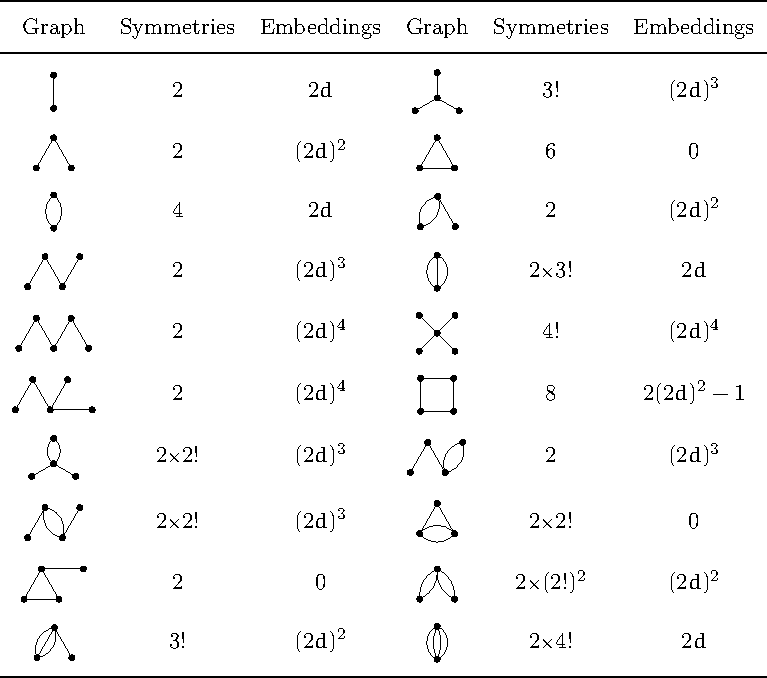
\includegraphics{embedding_and_symmetry}
  \end{center}
  \caption{Graphs with up to four bonds with symmetry factor and the embeddings
  on a $d$ dimensional square lattice.}
  \label{tab:graphs_embeddings}
\end{table}
%
A table of the four bond graphs with symmetry factors and embeddings on a square
lattice can be found in \tabref{tab:graphs_embeddings}. When we later
extrapolate the graphical methods to the effective theory we will see that these
are all graphs needed to carry out a computation to order $\kappa^8$.

\subsection{Cluster expansion for the effective theory at LO}

\subsection{Application to the effective theory, graph embeddings}

\section{Analytic resummation} \label{sec:analytic_resummation}
\section{Observables} \label{sec:evaluation}
\section{Large \texorpdfstring{$N_c$}{Nc} limit} \label{sec:large_nc_study}
\section{Yang Lee Zeros} \label{sec:yang_lee_zeros}
